\documentclass{beamer}

\usepackage{listings}
\usepackage{syntax}
\usepackage{amsmath}

\lstset{
  frame=none,
  xleftmargin=2pt,
  stepnumber=1,
  numbers=left,
  numbersep=5pt,
  numberstyle=\ttfamily\tiny\color[gray]{0.3},
  belowcaptionskip=\bigskipamount,
  captionpos=b,
  escapeinside={*'}{'*},
%  language=haskell,
  tabsize=2,
  emphstyle={\bf},
  commentstyle=\it,
  stringstyle=\mdseries\rmfamily,
  showspaces=false,
  keywordstyle=\bfseries\rmfamily,
  columns=flexible,
  basicstyle=\small\sffamily,
  showstringspaces=false,
  morecomment=[l]\%,
}
\begin{document}
\section{Introduction}
\begin{frame}
\frametitle{Overview}
\begin{itemize}
\item Implementation language: Haskell
\item Parser combinators
    \begin{itemize}
    \item Our own implementation
    \item Non-deterministic
    \item Handles errors (expected one of ... got ...)
    \end{itemize}
\item Split scan and parse phase
    \begin{itemize}
    \item Scanner implemented with parser combinators
    \item Recursive descent parser.
    \end{itemize}
\item Generally works great, but bad performance on some inputs (nested parenthesis)
\end{itemize}
\end{frame}

\section{Combinators}
\begin{frame}[fragile]

\frametitle{Parser Combinators}

\begin{itemize}
\item Parser combinators as presented in class.
\item With Haskell we only need \lstinline{bind}, \lstinline{pure}, and \lstinline{<|>}. We get a bunch of other stuff for free. Simple!
\item Until we want to handle errors!
\end{itemize}

\begin{lstlisting}
instance (Ord t) => Monad (Parser t) where
    (>>=) p f = Parser (\ts -> 
        case runParser p ts of
            (Error e) -> Error e
            (Success res1) -> foldl1 combineParses $
                fmap (\(a, ts2) -> runParser (f a) ts2) res1
            (Uncertain e res1) -> foldl combineParses (Error e) $
                fmap (\(a, ts2) -> runParser (f a) ts2) res1
            )
\end{lstlisting}

\end{frame}

\begin{frame}[fragile]

\frametitle{Error handling}

Combining parse results of the same type is simple:

\begin{lstlisting}
combineParses (Error e1) (Error e2) = Error (combineErrors e1 e2)
combineParses (Success m1) (Success m2) = Success (m1 <> m2)
combineParses (Uncertain e1 m1) (Uncertain e2 m2) =
    Uncertain (combineErrors e1 e2) (m1 <> m2)
\end{lstlisting}

The concept behind uncertain:
\begin{figure}
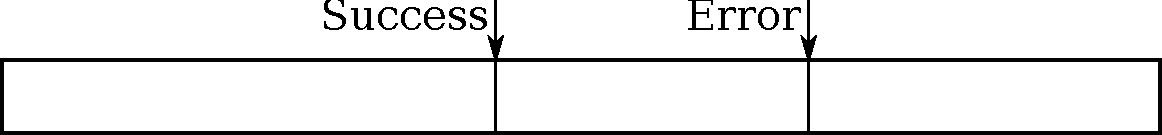
\includegraphics[width=10cm]{drawing}
\end{figure}
In this case we want to store both the success and the error.

Combining different types of parse results needs some consideration.


\end{frame}

\section{Scanning}
\begin{frame}[fragile]
\frametitle{Scanning}

\begin{lstlisting}
scanner = catMaybes <$> 
    (many $ (whitespace <|> symbol <|> intLit <|> ident)) 
\end{lstlisting}

\begin{itemize}
\item produces \lstinline{Maybe} values, so we can ignore white space.
\item Each sub parser uses the eager function to produce longest match.
    \begin{itemize}
    \item \lstinline{eager} gives the first success. This is used to get the longest possible symbol.
    \item \lstinline{(eager . many)} will give the longest match. This is used to get the longest identifier/integer literal/white space sequence.
    \end{itemize}
\item Identifiers are converted to keywords after they have been scanned.
\item We need to do \lstinline{scanner <* eof} to avoid getting every prefix of the token list.
\end{itemize}
\end{frame}

\section{Parsing}
\begin{frame}
\frametitle{Parsing}
\begin{itemize}
\item Recursive decent parser taking a list of tokens and returning an AST.
\item Uses the parser combinators. Relatively straight forward.
\item The hard part is precedence and associativity.
\end{itemize}
\end{frame}

\begin{frame}
\frametitle{Precedence}
Done as presented in the lecture, but we need to generalize a bit:
\begin{align*}
\text{exp}_n ::=&\ \text{exp}'_n\ \text{exp}''_n \\
\text{exp}'_n ::=&\ \text{exp}_{n+1} \\
\text{exp}''_n ::=&\ \text{op2}_n\ \text{exp}_n  \\
    | &\ \epsilon
\end{align*}
Because we use parser combinators we can parameterize over $n$.

At the highest level of precedence, we don't go further, instead we parse the other expressions types
\begin{align*}
\text{exp}'_{max} ::=&\ \ldots \\
    | &\ \text{op1}\ \text{exp}'_{max} \\
    | &\ \ldots
\end{align*}
Note that unary operators binds as tight as possible.
\end{frame}

\begin{frame}[fragile]
\frametitle{Associativity}
\begin{itemize}
\item The grammar from the previous slide returns right associative parse trees for all precedence levels.
\item Often we want a precedence level to be left associative (According to our understanding associativity only makes sense per precedence level, not for individual operators)
\item This cannot be done in the grammar.
\end{itemize}
\end{frame}
\begin{frame}[fragile]
\frametitle{Associativity}
...But we can still try notate it differently to get the idea across:
\begin{align*}
\text{exp}_n ::=&\ \text{exp}'_n\ [ \text{op2}_n\ \text{exp}_n ] \\
\text{exp}'_n ::=&\ \text{exp}_{n+1} 
\end{align*}
If we have a first expression, \lstinline{x} and a list of operator-expression pairs \lstinline{oxs}. We can do the following fold to get a left associative AST.
\begin{lstlisting}
foldl (\e1 (op, e2) -> Op2E op e1 e2) x oxs
\end{lstlisting}

To do the right fold we need a list of expression-operator pairs and the \emph{last} expression to do the fold. This is quite easy to achieve with a bit of massaging. 
\end{frame}

\section{Tests}
\begin{frame}
\frametitle{Tests}

\begin{itemize}
\item We have verified that the parser works on some of the given example programs.
\item Every well typed AST is syntactically valid, so we should be able to automatically generate test cases with QuickCheck.
\end{itemize}

\end{frame}

\section{Extra}
\begin{frame}
\frametitle{Extra stuff}
\begin{itemize}
\item We have a printer that will print an ASCII tree drawing of an AST implemented using generic programming and the \lstinline{drawTree} function of Data.Tree.
\end{itemize}
\end{frame}
\begin{frame}
\frametitle{Things that does not work yet}
\begin{itemize}
\item It is possible to cause the parser to backtrack a lot in some cases (nested parenthesis). Should be easy to fix by left factoring the grammar.
\item We don't have comments or character literals implemented.
\item Pretty Printing?
\end{itemize}
\end{frame}
\end{document}
